
\section{Methodology}
\label{sec:methodology}

	This section outlines our system design to overcome the targetted problem of distributed state sychronization design. We propose a distributed server model (see Figure~\ref{figure:server-models}(b)) to enable better failure handling in our system. In this model,the clients are paired with the servers that are running on the same machine to share their fate. The paired server validates the actions performed by corresponding client and process it further if the actions are found valid. Following subsections will discuss each component in the proposed architecture in detail.

\begin{figure}[ht]
	\centering
	\begin{tabular}{c c}
		
		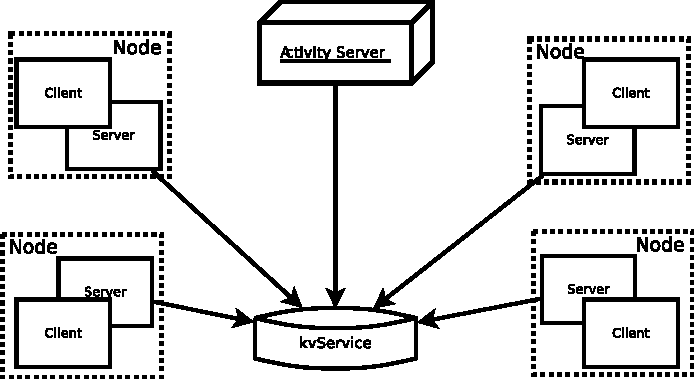
\includegraphics[width=0.52\linewidth]{../images/client-distributed-server-model-Activity-crop.pdf} &
		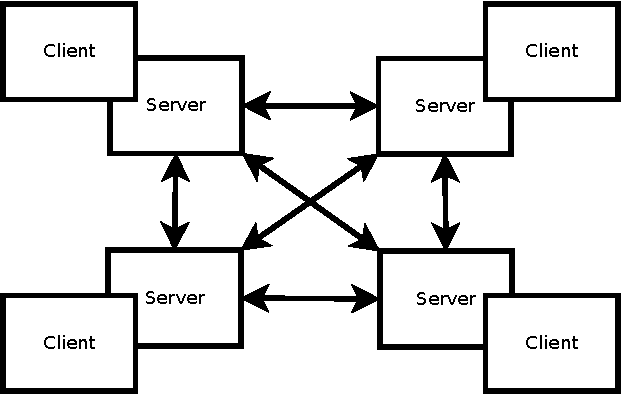
\includegraphics[width=0.40\linewidth]{../images/client-distributed-server-model-crop.pdf} \\
		(a) & (b)
	\end{tabular}
	
	\caption{\label{figure:server-models} The first figure (a) shows servers interation with \activityServer and \kvService. In this figure all of the servers periodically update their entry in the \kvService and the \activityServer periodically publish a list of online servers. The interation between \activityServer and servers only happens at the time joining In the second figure (b) shows server-server interactions in general.}
\end{figure}


\subsection{The Client}

	In general sense, a client provides an interface to the user/player, through which a player can give command to his character (we refered it as agent) in the game. The client runs a local version of the game, where the player's commands are executed. The commands executed by player on his agent produce changes in the state of the agent. 
	
	Each client in the system is paired up with a server (called as \localServer) which act as a proxy to all distributed servers in the system. Every change in the state of agent is forwarded to the \localServer. 
	
\subsection{The (Local) Server}

	The \localServer also runs its own independent version of the game. The state of game at \localServer is guided in coordination with rest of the \localServers in the system. The purpose of \localServer is not just to reduce message passing but also to act as a validator/authority over client's action, to prevent malicious client from propagating invalid information.The authoritative server for a particular client depends on the event/action being processed. Any client request is first forwarded to its \localServer where it is validated against the current state of game running at \localServer. The request is processed further only if the requested action is found valid, else the action is rejected by the \localServer. 
	
\subsection{The Activity Server}
	The purpose of \activityServer is to support the architecture of the system, which includes allowing a new node to join the system and publishing the list of nodes which are currently online. The \activityServer doesn't do any kind of game simulation niether get involves in game semantic actions.

\subsection{The Key-Value Service}
	The \kvService is a key-value service which act as a communication channel among different system components. The sole purpose of this service is to help the \activityServer to maintain the system. The nodes periodically update their entry in the \kvService and based on those entries, the \activityServer publish a list of nodes which are currently active. This list is later fetched by the nodes to know which all nodes are currenly online.

\subsection{ARM Game}

	ARM Game is an Asynchronous Real-time Multiplayer Game. It consists of two very basic actions for the players (charactrized as agent in the game). The first action is Move which is represented as \move{\agent}{\position}, where the first argument represents the agent intended to move and the second argument is its new proposed position. The other action is Fire which is represented as \fire{\position}{\direction}, where the first argument represents current position of the agent firing the shot and the second argument represents the direction in which the shot is fired.
	
	In order to simulate the game, information is needed on the other agents in the game. The required information corresponding to each agent is called as \agentstate. The attributes of \agentstate are shown in Table~\ref{table:gamestate-struct}. A collective database storing \agentstate of all agents in the game is  known as \gamestate.  
	
\subsubsection{Protocol and Messaging}

	The clients send request to their \localServers. The \localServer validates the request againts its own version of \gamestate. If \localServer finds it valid, then only the request is forwarded to the authoritative \localServers over that agent for that particular action. All communications are asynchronous without acknowledgements. We used JSON to facilitate messaging is the system.


	
